% Chapter 1

\chapter{Prototype II} % Main chapter title

\label{prototype2chapter} % For referencing the chapter elsewhere, use \ref{Chapter1} 

\lhead{Chapter \ref{prototype2chapter}. \emph{Prototype II}} % This is for the header on each page - perhaps a shortened title

%----------------------------------------------------------------------------------------
\section{Prototype Development Iteration II}\label{prototype2descr}
I started the next iteration of prototype development that aimed to improve the first prototype described in Chapter \ref{prototype1chapter} (Prototype I). In the second prototype, the emphasis was more on improving support for the three psychological needs from self-determination theory \citep{ryan2000:self}, which are relatedness, competence and autonomy. I replaced Facebook social plug-ins with features that would allow users to directly comment on or like each other. Facebook social plug-ins failed to integrate seamlessly with the app, since the network signal was poor in the area where I conducted the previous evaluation reported on in Chapter \ref{prototype1chapter}. Therefore, users failed to load them into the app. In addition, the improved system implemented SMS reminders and feedback instead of Facebook-based reminders. The idea in the second prototype was to design challenges that promote collaboration between intermediaries and beneficiaries; as a result, I did improve the design of the challenges to encourage an intermediary and a beneficiary to work together towards the self-monitoring of health for the beneficiary participant. In the evaluation of the first prototype, I observed that collaborative discussions between members of a pair  with prior social relationship, enhanced engagement and made the app more fun to use. Therefore, the design of the second prototype retained the single user interface shared by a pair, to make the collaboration more practical. The new system is shown in Figure \ref{figure:prototype_2_screens}.

\begin{figure}[htbp]
  \centering
    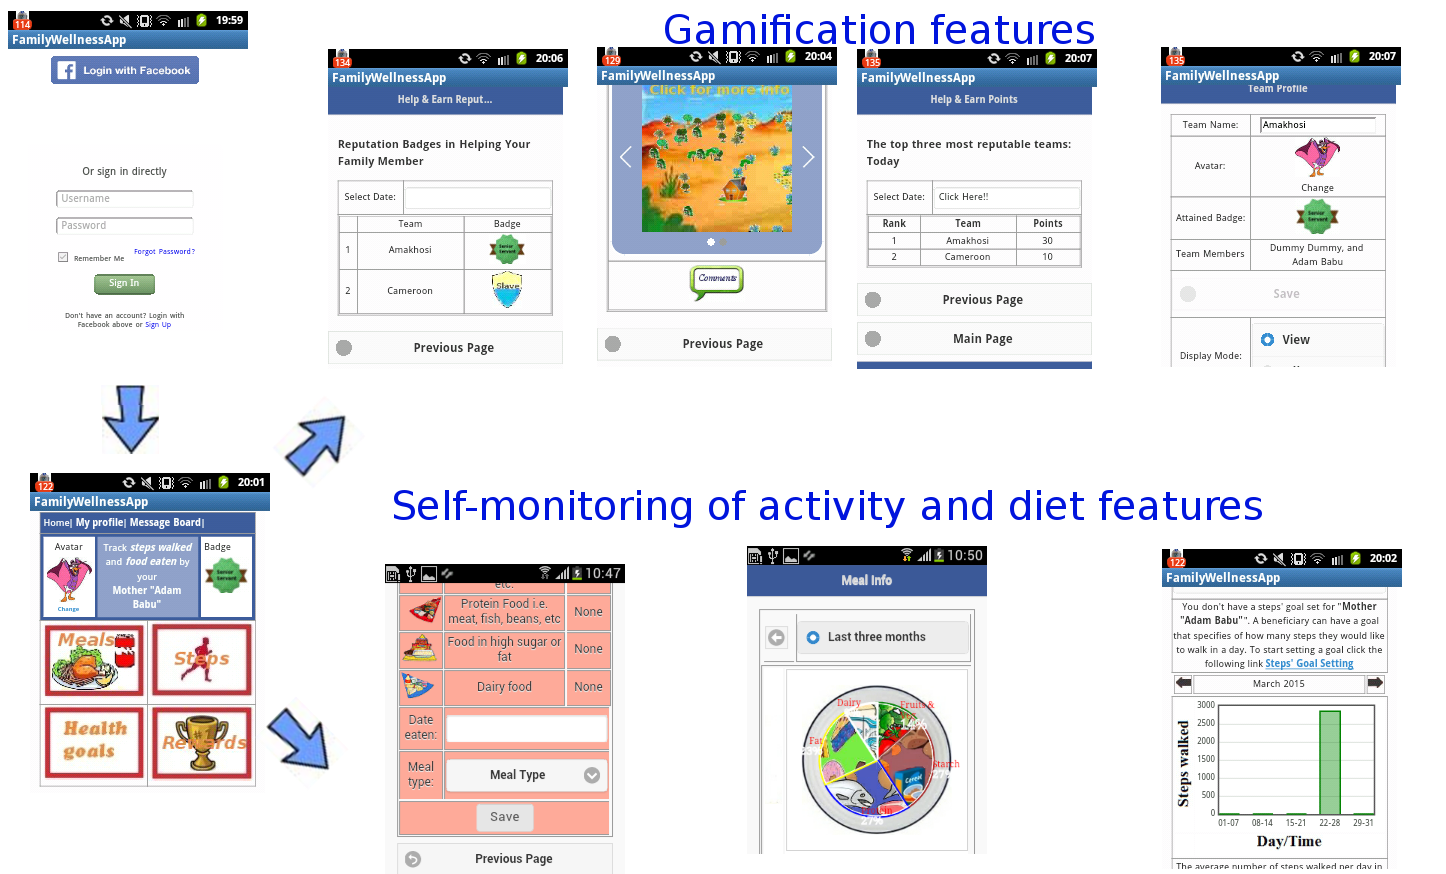
\includegraphics[width=0.8\textwidth]{Figures/Version2/Prototype2Screenshots.png}
    \rule{35em}{0.5pt}
  \caption{Sample screen-shots of the second prototype.}
  \label{figure:prototype_2_screens}
\end{figure}

In this improved prototype, some features remained the same as or slightly improved from, the first prototype. For instance, the journal for
self monitoring of nutrition and physical activity, was only improved to give users the flexibility in navigating across the recorded data by using different intervals of time: daily, weekly or monthly summaries, for physical activity and nutritional components of meals.

This prototype also consisted of a leaderboard as in the previous prototype. In this leaderboard, each team (a pair of users) is ranked based on their points, which are determined using three factors: frequency of app usage, beneficiary's footsteps count, and recorded nutritional components of meals consumed by the beneficiary. However, there is a difference between the leaderboard reported on in the previous chapter and this one: the current leaderboard contains a few information (only displays names and points, for participating teams); in the first prototype, the leaderboard contained points, badges and participant names. Points are more meaningful in a leaderboard as they promote competition with others; badges can be used to promote both competition with self and competition with others. Therefore, I as the developer, decided to separate badges and points to stand independently, on their own interfaces.  

In the improved prototype, badges are awarded sequentially to teams that achieve two important milestones (challenges -- coded in the app): a team must have at least a certain number of both footsteps and days in using the app, that are required to attain a higher badge (by one position) than the current badge. The script that awards teams with new badges was set to run at most once a day and used the predefined challenges similar to the ones in Table \ref{table:badges}; any team that solves the current challenge is then promoted to the next higher badge. These badge-attainment requirements are more stringent than the ones used in the first prototype, where the incremental process was not followed, as a result, teams could skip intermediate badges in between and get to the highest badge that corresponds to their current performance. This made the badge challenge easier to attain within a few days as it was observed in the case of Jabulani and his mother (Chapter \ref{prototype1chapter}). The improved set of challenges required a much longer pair's commitment to the intervention, to reach the highest badge (Queen/King). Therefore, the new rules increased the difficult level of the presented challenges. Each team had their badge displayed in two places: in the top right corner of the main screen and at a separate board that also displayed badges for other teams.
\begin{table}[h!]
  \begin{center}
    \caption{Examples of badge challenges in the app.}
    \label{table:badges}
	\begin{tabular}{|l|l|p{3cm}|p{4cm}|}
		\hline
		Status &Badge &Frequency of app usage (days)&Daily average number of footsteps\\
		\hline
		Queen/King&
\includegraphics[scale = 0.75]{Figures/badges/king.jpg}&18&10000\\
		\hline
		Princess/Prince&
\includegraphics[scale = 0.75]{Figures/badges/prince.jpg}&16&9000\\
		\hline
				Grand Master&
\includegraphics[scale = 0.75]{Figures/badges/grandmaster.jpg}&12&7000\\
		\hline
		 .&.&.&. \\ 
		 .&.&.&. \\   
		 .&.&.&. \\ 
		 .&.&.&. \\
		 .&.&.&. \\
		 \hline
		Servant&
\includegraphics[scale = 0.75]{Figures/badges/servant.jpg}&1&2500\\
		\hline
		Slave&
\includegraphics[scale = 0.75]{Figures/badges/slave.jpg}&0&\textless 2500\\
		\hline
	\end{tabular}
  \end{center}
\end{table} 

One observation from the first evaluation (Chapter \ref{prototype1chapter}) is that, the process of recording meals was not as popular as, was the tracking of the steps, because, it did not indicate any pattern in arousing the interest of the participants. One possible reason for this is the weak link between the process of recording meals and the resulting rewards in gamification, as a result, pairs could not offer insights on engagement with this feature, only to focus on the steps. Therefore, I improved challenges for the fish tank and the botanical garden, to bring engagement with the process of diet self-monitoring. The improved design aimed to also promote healthy eating. I made the process of diet self-monitoring more salient by linking it to the vitality of virtual pets (fish and trees): the number of trees in the garden or fish in the tank were determined by the current team's badge and the number of meals recorded. There was a bonus awarded for meals containing portions of fruit and vegetables. This bonus is used to improve the appearance of both plants in the garden and fish in the tank. Therefore, in this new design, steps, frequency of app usage and more specific, frequency of recording meals, all three contributed to both the growth of trees in the garden and fish in the tank; the frequency of app usage and the captured footsteps, contributed indirectly through badges. 

The last additional improvement in the app, aimed to support autonomy: a team is now able to edit their team's name and change their avatar.

I did  specify the rules for engaging with gamification as part of the user manual. But the system also sent periodic SMS hints to pairs, to remind them, what they need to do, to master the presented challenges. These messages were tailored with the name of the intermediary participant. For instance: ``\emph{Tip of the day: Hey Zizile, every recorded meal by your aunt can give you points to buy food for your fish...[Family Wellness App]}''. 
 
\section{Prototype Evaluation Description}
In this evaluation, I had planned to recruit another group of participants. The NGO facilitated access to a group which resided in a different area of Philippi from where evaluation of the first prototype was conducted. The plan, however, did not materialize, as the NGO suggested that we look for a different group, because the group they were working with expressed concerns regarding safety issues after they heard that they were going to be given phones to use throughout the evaluation period. The NGO was concerned about the safety of researchers, since rumours had spread throughout the community that someone was going to bring phones to that area. This posed risks to both prospective participants and the researcher, and highlights the limitations and dangers of doing smartphone-based interventions in low-income areas~\citep{Molapo2015}. 

In order to proceed, I revised the plan, and in the process, found another low-income township called Langa, more modern, not far from the central business district (Cape Town), and safer compared with Philippi. 

A research facilitator who was a resident of Langa helped with the recruitment process. This time, I came up with more stringent recruitment criteria than the previous evaluation (Chapter \ref{prototype1chapter}). I introduced one of the criteria as having intermediaries that cohabit or live near the beneficiaries. Preference was given to schoolgoing children as they were more likely to be interested in gamification. The research assistant managed to recruit a total of nine adult participants for the study: three males and six females, with an average age of 49.3 years (standard deviation of 7.9 years ). Each adult participant brought one intermediary participant and formed a pair. There were three male and six female intermediary participants, with a mean age of 14 years (SD=4.3). Eight of the adults  were relatives/familial relatives of intermediary participants, while the remaining adult was a tenant of her intermediary's grandmother. Eight of the intermediary participants were schoolgoing children.

Prior to commencement of the study, I gave out information about the study to both beneficiary and intermediary participants, informed them that the study's cellphone would be collecting their information related to usage of the app, steps walked, and recorded nutritional components of meals consumed by beneficiary participants. I informed them that the collected information would be transferred to a computer at the University of Cape Town. All participants who were not minors signed informed-consent forms, while minors signed assent forms that were also signed by their guardians/parents.

Once consent and assent forms were signed, one day was allocated to training intermediary participants how to use the app. After the training, I provided each pair with one Android phone (Samsung
GT-S5300), installed with two native apps. The first app was a pedometer (the same given in Chapter \ref{prototype1chapter}), which displayed no useful information other than raw steps data. The pedometer's task was to send these steps to a server so that they could be presented  and viewed in a better format through a web application. The second app provided a link to the web application. One small observation from the previous evaluation reported on in Chapter \ref{prototype1chapter} (Prototype I), it was difficult for users to remember the URL for the web app, therefore a native link provided the easy way to access the app.

In order to encourage participation, each beneficiary participant received ZAR40 ($\approx$USD4) worth of airtime four times in a period of three weeks: ZAR160 ($\approx$USD16) in total. To encourage participation of intermediary participants, the research credited each pair with 300MB of data to use on the Android phone, as it was expected that intermediaries would borrow phones to access other things on the Internet that were beyond the prescribed uses. Providing data bundles was so as to avoid the problem of intermittent usage due to lack of data as observed in the previous chapter.

I deployed the app in the field for three weeks and at the end I conducted an evaluation. The next subsection provides the description of the evaluation.
\section{Prototype Evaluation Methods}
The evaluation relied on two approaches: (1) collecting user logs and (2) interviews. As, all respondents were familiar/comfortable with English, I conducted all the interviews in English. I interviewed a total of three intermediary participants, and five beneficiary participants. These were the only participants that I could reach during the time of interviews. Each short interview lasted for 15 minutes at most. Pseudonyms have been used in findings from the interviews in order to protect the identities of the participants. On reporting the age of participants in interview excerpts, the notation \emph{yrs} refers to years. When the participant's name is introduced or appearing within text (including excerpts) for the first, their age and gender are also mentioned. When participants are mentioned without their age or gender, it implies that they have already been introduced before. 
\section{Findings}
The key findings were based on social technical settings and motivational strategies that influenced usage of the app. Some of the findings from this chapter together with findings from the previous chapter (Chapter \ref{prototype1chapter}) have appeared in a conference paper that I co-authored \citep{katule2016leveraging}.

In this context, intermediaries were very useful in facilitating access on behalf of their respective beneficiary users; hence intermediaries were acknowledged as having expertise that beneficiaries did not have (Table \ref{table:skilledintermediaries}).

\begin{table}[h!]
\renewcommand{\baselinestretch}{1.5}
  \begin{center}
    \caption{Excerpt: an example of how intermediaries trusted as experts by beneficiaries.}
    \label{table:skilledintermediaries}
	\begin{tabular}{|l|C{12cm}|}
		\hline
		No.&Comment\\
		\hline
		1.&\userquote{\textbf{Dlamini}, a male beneficiary, 72 yrs} {``When it comes to the app, I give it to him [\textbf{Vuyo}, a male intermediary, 10 years old]. He is the mastermind on it. All I tell him is just what happened during the course of the day, the meals were as follows, and he is the one that manoeuvres all the stuff.''} \\
		\hline
	\end{tabular}
  \end{center}
\end{table} 

There were two main factors that were crucial in facilitating intermediated use in the context of this evaluation. The subsections below have highlighted these factors.

\subsection{The Role of a Familial Relationship in the Intervention}
As noted in the previous chapter (Chapter \ref{prototype1chapter}), a parent-child relationship may be important in the implementation of such an intervention. In this case, a prior social relationship was also very important. Intermediaries who were working with their parents were eager to support their parents because they cared about them. 

I clustered usage by each pair to its respective relationship type as shown in Figure \ref{figure:relation}. There were three types of relationships: parent-intermediary, relative-intermediary, and not related, with four, three and one as their respective number of pairs. I measured usage within each relationship through three dimensions: (1)~the mean number of days for all pairs; (2)~the average number of sessions per pair; and (3)~the average number of clicks per pair. As a result, I observed more usage for pairs with a parent-intermediary relationship. 
\begin{figure}[htbp]
  \centering
    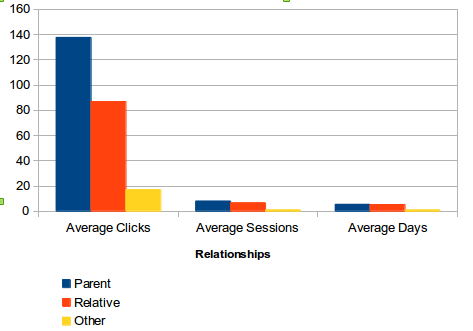
\includegraphics[width=0.7\textwidth]{Figures/relationships.png}
    \rule{35em}{0.5pt}
  \caption{Usage in three groups of relationships~\citep{katule2016leveraging}.}
  \label{figure:relation}
\end{figure}
In the case of parent-intermediary or relative-intermediary relationships, negotiation for interaction that was initiated by beneficiary users was more possible because of the nature of the prior social relationship. In cases of a good prior social relationship, requests from beneficiaries were always successful most of the time. For instance, \textbf{Zandiwe}, \emph{a beneficiary user, a 50-year-old woman}, was working with her sister's daughter. In another case, \textbf{Lulama}, \emph{an intermediary user, a girl aged 20}, was working with her mother, \textbf{Nokhanyo}, \emph{57 years old}. The two cases are presented in Table \ref{table:negotiations}

\begin{table}[h!]
\renewcommand{\baselinestretch}{1.5}
  \begin{center}
    \caption{Excerpts: examples of how a good prior social relationship gave an advantage to beneficiaries when negotiating for intermediated use.}
    \label{table:negotiations}
	\begin{tabular}{|l|C{12cm}|}
		\hline
		No.&Comment\\
		\hline
		1.&\userquote{\textbf{Zandiwe}, a beneficiary} {``I used to call Lindiwe [an intermediary, 16 years of age] like `Lindiwe, there is something that I don't understand'. Or I call her the day before when I walk for a long time, I call her to come and help me some way somehow.''} \\
		\hline
		2.&\userquote{\textbf{Lulama}, an intermediary} {``My mother was the one who was pushing me, let’s do it, let’s do it. And we spent more time together. But we are always together around that time; I do the app at around eight o'clock at night. So we talk more than before because she would ask `How am I doing on this?' ''}\\
		\hline
	\end{tabular}
  \end{center}
\end{table} 

There were instances where a beneficiary user would request assistance at the time when the intermediary was either resting or occupied with other activities or felt that there was no urgency in fulfilling such a request. However, a social relationship still played a role in getting intermediaries to immediately attend to such requests; this was possible, due the empathy on the side of intermediaries; hence such intermediaries had more sense of being accountable to their family members regardless of whether their autonomy was violated or not (Table \ref{table:autonomy_vs_relationship}). The excerpt by Lulama, demonstrates that she was aware that her mother had limited skills in operating technology and it was a sufficient rationale to give that kind of assistance, because she cared for her. 

\begin{table}[h!]
\renewcommand{\baselinestretch}{1.5}
  \begin{center}
    \caption{Excerpts: examples for intermediaries' inclination towards balancing between the need for own's autonomy and the need to preserve an existing relationship with their beneficiaries.}
    \label{table:autonomy_vs_relationship}
	\begin{tabular}{|l|C{12.5cm}|}
		\hline
		No.&Comment\\
		\hline
		1.&\userquote{\textbf{Nokhanyo}, a beneficiary} {``We like to fight each other. Sometimes she [\textbf{Lulama}] is lazy to record. I say to her `come up come up you didn’t do your job'. She would say `I am tired from work'. But she would wake up and do everything for me.''} \\
		\hline
		2.&\userquote{\textbf{Lulama}, an intermediary} {``I am helping her so it [the app] has to mean a lot to me.~I am helping her (Nokhanyo) because she doesn't know anything. She is like `What is this?' This is how you do this. She is like `Ooh okay'. So it [the app] means a lot to me because I am helping someone I care about.''}\\
		\hline
	\end{tabular}
  \end{center}
\end{table}  

Another observation from pairs with a parent-child relationship was that  intermediaries demonstrated a sense of being co-owners of the information from the system, because of being absorbed by the experience of interacting with certain motivational affordances in the app. For instance, Lulama used the terms ``we'' or ``our'' repeatedly to describe actions that needed to be carried out by her beneficiary user as shown in Table \ref{table:coownership}. Here it means such an individual's actions are perceived as belonging to the team and not to an individual only. Such cases demonstrated a sense of collaborative ownership of information in the app, which promoted collaboration in using the app. A sense of collaborative ownership was the result of both prior social rapport and engagement from motivational affordances.

\begin{table}[h!]
\renewcommand{\baselinestretch}{1.5}
  \begin{center}
    \caption{Excerpt: an example of an intermediary showing a sense of being a co-owner of the process and outcome in using the app.}
    \label{table:coownership}
	\begin{tabular}{|l|C{12.5cm}|}
		\hline
		No.&Comment\\
		\hline
		1.&\userquote{\textbf{Lulama}, an intermediary} {``When I saw the garden I was like `yeah, our garden is looking beautiful. Let's do more. Let's take more steps. Let's eat more veggies, because it is the veggies and fruit that are important'.''} \\
		\hline
	\end{tabular}
  \end{center}
\end{table} 
 
From a sense of co-ownership, there was a collaborative reflection. Collaborative reflection happened after negotiation to initiate interactions was successful. Negotiations would be initiated within a pair by either member of a pair. Once a negotiation to initiate interaction was successful, then intermediary users navigated through the app. In the process of navigating through the app, anything intermediaries found interesting would be shared with their respective beneficiary users (Table \ref{table:proximatetranslation}).

\begin{table}[h!]
\renewcommand{\baselinestretch}{1.5}
  \begin{center}
    \caption{Excerpt: an example of how intermediaries enabled proximate translation of intents to interact with the app.}
    \label{table:proximatetranslation}
	\begin{tabular}{|l|C{12.5cm}|}
		\hline
		No.&Comment\\
		\hline
		1.&\userquote{\textbf{Nokhanyo}, a beneficiary} {``I didn't use the app. Lulama used the app. I can't use it. She just shows me and then she presses everything.''} \\
		\hline
	\end{tabular}
  \end{center}
\end{table} 

This kind of interaction sparked a conversation between the two users (members of a pair).~As a result of sharing information between members of a pair, there was a collaborative reflection that increased engagement and promoted a bond between two members of a participating pair through motivational affordances that were either directly situated in the app or indirectly situated in the app (i.e. social comparison among beneficiaries who had formed an informal social support group). Through a collaborative reflection, there were attempts by intermediaries to  persuade their respective beneficiaries to do what would be beneficial in getting virtual rewards for the team (i.e. walking more steps) as shown in Table \ref{table:persuaders}.

\begin{table}[h!]
\renewcommand{\baselinestretch}{1.5}
  \begin{center}
    \caption{Excerpt: an example of how intermediaries posed as persuaders for their beneficiaries.}
    \label{table:persuaders}
	\begin{tabular}{|l|C{12.5cm}|}
		\hline
		No.&Comment\\
		\hline
		1.&\userquote{\textbf{Lwazi}, an intermediary, a boy aged 14 yrs} {``I tell her [his mother] like every two or three days `you must go to town to see if you can find a couple of clothes good for me; you will take the steps also'. She takes the phone with her. She puts the phone in her pocket.''}\\
		\hline
	\end{tabular}
  \end{center}
\end{table}

And such intermediaries did not persuade solely for attaining virtual rewards; they also cared about the health of the people they were helping. This phenomenon was observed in two pairs as shown in Table \ref{table:caretakers}.

\begin{table}[h!]
\renewcommand{\baselinestretch}{1.5}
  \begin{center}
    \caption{Excerpts: examples for intermediaries posing as caretakers for their beneficiaries.}
    \label{table:caretakers}
	\begin{tabular}{|l|C{12.5cm}|}
		\hline
		No.&Comment\\
		\hline
		1.&\userquote{\textbf{Nokhanyo}, a beneficiary} {\enquote{Sometimes she used to shout at me. \enquote{No, no you didn't eat that thing. Tell me what you ate in the morning. I saw you eating this. It seems there is nothing for fruits, peanuts. You must remind me to check you}.}}\\
		\hline
		2.&\userquote{\textbf{Lwazi}, an intermediary}{``It [the app] was really good because my mother was limiting herself on stuff like pies and fat food. I would tell her `Don't eat this; don't eat that'. She wasn't eating much vegetables but I was encouraging her to eat vegetables.''}\\
		\hline
	\end{tabular}
  \end{center}
\end{table}

For those pairs that did not have a parent-child relationship, interactions between members were minimal or absent except for cases where an intermediary was motivated by access to the intervention's phone or motivation affordances provided by gamification. Nevertheless, in such cases a prior social relationship, played a role, i.e. relative-intermediary (child), although it was not as strong as a parent-intermediary relationship. In a parent-child relationship the bond was much stronger to the point where intermediaries had authority in persuading their respective beneficiary users. However, the relative-child relationship was better than the absence of a familial relationship. In such cases of relative-intermediary relationships, intermediaries would still provide infrequent help to their beneficiaries. Where there was no relationship between an intermediary and beneficiary, even infrequent help was not available, e.g. \textbf{Anele} (a beneficiary user, a 47-year-old woman, who was working with the granddaughter of her landlord; hence they did not have a familial relationship. Anele shared her frustrations that the child she was working with was not being cooperative.  Every time she requested help, her intermediary claimed to be busy and kept on procrastinating by saying they would do it the next day, and when that day came it was the same thing. Therefore, a familial relationship was an integral component in mediating motivation of some intermediaries to help in this context.   
\subsection{Sources of Motivation for the Two Sets of Users}
In cases where both users of a pair were motivated to use the app and there was a prior social relationship between them, the pair tended to interact in a more playful manner, which brought the two users closer that they were before using the app. This happened when an intermediary was sharing the information to a beneficiary user. In that process of sharing, the interaction was enjoyable and less tense. The excerpt in Table \ref{table:collaborativereflection} describes how the interaction  between members of one pair was enjoyable when the two users were collaboratively engaging with the app. Lindiwe shows excitement upon seeing steps walked by Zandiwe. 

\begin{table}[h!]
\renewcommand{\baselinestretch}{1.5}
  \begin{center}
    \caption{Excerpt: an example of how collaborative reflection enhanced engagement.}
    \label{table:collaborativereflection}
	\begin{tabular}{|l|C{12.5cm}|}
		\hline
		No.&Comment\\
		\hline
		1.&\userquote{\textbf{Zandiwe}, a beneficiary} {` When she [\textbf{Lindiwe}, a girl aged 16 yrs] got time, when she is done with her homework she comes and sees the app. And then laughs at me like `Yo yo yo [an interjection for Xhosa speakers to express the feeling of amazement by something], you can walk yo yo yo', like `you walked a lot today' and what what [referring to other things said by Lindiwe].''}\\
		\hline
	\end{tabular}
  \end{center}
\end{table}

Also, Nokhanyo mentioned how interaction with her daughter was accompanied by laughter during the exchange of information retrieved from the app. This playful environment fostered relatedness and made it easier for the two users from a pair to collaborate and continue engaging with the app. 

However, in engaging with the app, intermediaries and beneficiaries had different motivational goals. Intermediaries were interested in pursuing a goal related to either steps or eating healthily for their beneficiaries in order to achieve rewards in gamification.~For beneficiaries, the primary goal was to achieve more steps for the purpose of informal comparisons with others or for instrumental value to their health. The subsections below expand further on these different sources of motivation.
\subsubsection{Sources of Motivation in Beneficiaries}
One of the factors that played a role in motivating beneficiaries was informal comparison of steps/diet. In the app, there was no feature that supported direct comparison of steps or diet. Instead, beneficiary participants who knew each other implicitly formed a social support group (Table \ref{table:informalsupport}) . In this support group, they interacted with each other through either face-to-face meetings or SMS/voice. These interactions were centred around comparison of steps or diet among each other. Beneficiaries within social support groups were curious about how others were doing and expressed as much while conversing with the respective intermediary users.

\begin{table}[h!]
\renewcommand{\baselinestretch}{1.5}
  \begin{center}
    \caption{Excerpts: examples for existence of informal social support groups for beneficiaries.}
    \label{table:informalsupport}
	\begin{tabular}{|l|C{12.5cm}|}
		\hline
		No.&Comment\\
		\hline
		1.&\userquote{\textbf{Zandiwe}, a beneficiary} {``We [with Nokhanyo] were talking about what we ate. Like Tuesday I phone Nokhanyo to ask her `Did you eat a lot?'. She said `Not today' But she said she ate a lot the day before. It was Monday.''}\\
		\hline
		2.&\userquote{\textbf{Lulama}, an intermediary} {``She [Nokhanyo] would ask `I wonder how so and so is doing?'. She would ask them when she sees them. She wouldn't ask on the app.''}\\
		\hline
	\end{tabular}
  \end{center}
\end{table}

These kinds of social comparisons led to competition between beneficiary participants. Such competition was a consequence of how the app was utilized in the existing social context and not an intended goal of design, as participants extended comparisons beyond what the design of the app supported. Some beneficiary users had set their targets or goals in order to perform better than beneficiaries from other teams within their social support group (Table \ref{table:comparisonbeneficiaries}).

\begin{table}[h!]
\renewcommand{\baselinestretch}{1.5}
  \begin{center}
    \caption{Excerpt: an example of how comparison for steps within the informal social support group steered competition.}
    \label{table:comparisonbeneficiaries}
	\begin{tabular}{|l|C{12.5cm}|}
		\hline
		No.&Comment\\
		\hline
		1.&\userquote{\textbf{Ndileka}, a female beneficiary user, 35 yrs}
{\enquote{I think I was in competition with steps [she is chuckling]. Because others would have said `Ooh I have walked', maybe we look at the thing [pedometer], it says 1900 steps [referring to steps walked by her peers]. And for me I will say \enquote{No, tomorrow I need to walk more than her because she walked 1900 steps. Then I need to walk 2500 steps}.}}\\
		\hline
	\end{tabular}
  \end{center}
\end{table} 

Also, some beneficiaries became interested in some of the gamification features after \emph{proximate translation by intermediary users} (Table \ref{table:bengamengage}). Therefore, intermediaries needed interpretation of what was going on in gamification in order for them to understand it.

\begin{table}[h!]
\renewcommand{\baselinestretch}{1.5}
  \begin{center}
    \caption{Excerpts: examples for beneficiaries' engagement with gamification through proximate translation of information in the app.}
    \label{table:bengamengage}
	\begin{tabular}{|l|C{12.5cm}|}
		\hline
		No.&Comment\\
		\hline
		1.&\userquote{\textbf{Lulama}, an intermediary} {``She [Nokhanyo] saw the garden. The first day she saw just the house and brownish. She is like `what is this'. I told her. She said `Aha! [expressing
dissatisfaction]. It must look green and healthy'. And then
she saw the garden again and said `It is looking good'.''} \\
		\hline
		2.& \userquote{\textbf{Lwazi}, an intermediary} {``She [his mother] doesn't understand the app. I just tell her that people are having ones twos threes (on the scoreboard and badges) and she laughs.''}\\
		\hline
	\end{tabular}
  \end{center}
\end{table} 

Therefore, the most motivating factors for beneficiaries were steps feedback (for challenging self) and comparison (competition) of steps with others. 
\subsubsection{Sources of Motivation in Intermediaries}
There are several factors that motivated intermediaries to use the app, apart from a prior social rapport. Factors that manifested in participants' responses include gamification features, effect of intervention's phones, and self-monitoring of steps. Some intermediaries nudged their beneficiary
users to do more steps or to eat healthily, so that their pairs would win rewards offered by gamified elements of the web app. The extent of nudging was evident in pairs with a parent-child relationship. Gamification features such as badges, a leaderboard and gardens mediated both competition with other intermediaries and competition with self as shown in Tables \ref{table:intermleadengage}.

\begin{table}[h!]
\renewcommand{\baselinestretch}{1.5}
  \begin{center}
    \caption{Excerpt: an example for the role of gamification in motivating intermediaries.}
    \label{table:intermleadengage}
	\begin{tabular}{|l|C{12.5cm}|}
		\hline
		No.&Comment\\
		\hline
		1.&\userquote{\textbf{Lwazi}, an intermediary}{``The app challenged me to compete [with others] because there was this lady I think it was Lulama. She was getting points and I was really stressed out because she was reaching the amount I was getting, so I was pushing hard to get there. But now I am second. If I was using the app so much, I was going to be number one but I am not using the app so much because my mother is not putting her SIM card on the phone....It's the same like a battle; you are battling with other people. So you must be on your toes with the app and see what is going on with your family.''} \\
		\hline
	\end{tabular}
  \end{center}
\end{table} 

Intermediaries were able to interpret some of the intentional motivational affordances that were aimed at persuading intermediary users to perform certain tasks on behalf of their respective beneficiary users. An example of such motivational affordances is where the size of the fish was related to how often meals consumed by a beneficiary user within a pair were recorded. When \textbf{Lwazi} (an intermediary user) was asked what the size of the fish in his tank was, his response was as follows: \emph{``They were medium sized because I wasn't really feeding them.''} By not feeding them he implied that he was not doing enough to record the meals eaten by his mother. This is an example of a connection that was made between playful interfaces and actual health self-monitoring behaviours. Other examples of how such motivational affordances motivated intermediaries are provided in Table \ref{table:intermgardenengage}

\begin{table}[h!]
\renewcommand{\baselinestretch}{1.5}
  \begin{center}
    \caption{Excerpts: examples of how intermediaries' reacted to challenges.}
    \label{table:intermgardenengage}
	\begin{tabular}{|l|C{12.5cm}|}
		\hline
		No.&Comment\\
		\hline
		1.&\userquote{\textbf{Vuyo}, an intermediary}{``When I had little trees it [the garden] encouraged me to record more meals''}\\
		\hline
		2.&\userquote{\textbf{Lulama}, an intermediary} {``When I saw the garden, I was like `Yeah, our garden is looking beautiful. Let's do more. Let's take more steps. Let's eat more veggies, because it is the veggies and fruit that are important'.''}\\
		\hline
	\end{tabular}
  \end{center}
\end{table} 

The findings also revealed unintentional persuasive effects that resulted from SMS reminders. In one context, three participants (one intermediary and two beneficiaries) were convinced that messages were sent by the researcher (myself). The system auto-generated messages tailored with the participants' names. The three participants perceived them as real messages forwarded by the researcher, who probably was following their performance and was trying to encourage them. For instance, in the case of \textbf{Nokhanyo} (a beneficiary user), every time she received a message she would call her daughter to come and see by telling her that it is from so and so (mentioning the name of the researcher). This caused \textbf{Lulama} (an intermediary user) to panic whenever she heard her mother call her about a received SMS. \textbf{Lulama} kept thinking that she had done something wrong.  In a different scenario, \textbf{Lwazi} (an intermediary user) thought that messages were sent by other participants through a message board that was on the app. Therefore, he passed these reminders on to his mother, saying that people were reminding them about eating healthily, and the mother always responded with laughter. \textbf{Lwazi} used these messages to encourage his mother to walk more steps and eat healthily.  

Apart from gamification features, the phone motivated intermediaries to participate, especially those who had a prior social relationship with their beneficiaries. Intermediaries were involved in tasks that were non-prescribed in the course of carrying out tasks within prescribed use. For instance, two intermediaries aged 10 and 14 had installed games on the intervention's phones that their parents had.  In another case, an intermediary user called \textbf{Lindiwe}, lived a distance from a beneficiary user \textbf{Zandiwe}, but she came all the way to use the phone and to interact with gamification.~\textbf{Zandiwe} was \textbf{Lindiwe}'s aunt (Table \ref{table:phoneeffect}).   

\begin{table}[h!]
\renewcommand{\baselinestretch}{1.5}
  \begin{center}
    \caption{Excerpt: an example for the effect of the study's phone in increasing intermediaries' engagement.}
    \label{table:phoneeffect}
	\begin{tabular}{|l|C{12.5cm}|}
		\hline
		No.&Comment\\
		\hline
		1.&\userquote{\textbf{Zandiwe}, a beneficiary} {``\textbf{Lindiwe} likes the phone too much. She is always here after school. She lives with my sister on the other side and she comes here every day. Sometimes I call her to come. We are closer than before. We always talk about the app while other people (relatives) are around. These people also got interested''} \\
		\hline
	\end{tabular}
  \end{center}
\end{table}

There was also the novelty effect of the self-monitoring tasks (diet's pie chart and steps' bar chart). Some intermediaries were excited to see visualization of information about people they cared about. For instance, one 10-year old intermediary, mentioned that steps were the most interesting of all the features. 

\subsection{Perceived Value in Using the Prototype}
The beneficiaries said they had gained knowledge about living a healthy lifestyle (Table \ref{table:benknowledge}).

\begin{table}[h!]
\renewcommand{\baselinestretch}{1.5}
  \begin{center}
    \caption{Excerpts: examples of how the app improved beneficiaries' knowledge.}
    \label{table:benknowledge}
	\begin{tabular}{|l|C{12.5cm}|}
		\hline
		No.&Comment\\
		\hline
		1.&\userquote{\textbf{Zandiwe}, a beneficiary} {``There are a lot of things I didn't know I now know, like how to eat. I know walking is very important. Because, you know, I am fat. When I stay on the bed the whole day, my blood doesn't circulate.''}  \\
		\hline
		2.&\userquote{\textbf{Ndileka}, a beneficiary} {``The app helped me because sometimes you don't realize you eat more carbohydrate than fruit. You just eat bread but you don't know that bread is carbohydrate. So when it says a large amount of carbohydrate, you know I am eating a large amount of carbohydrate. You think `Now I must eat more fruit than meat or less meat'. So for me automatically it helped me to think that I need to eat a large amount of fruit.''}\\
		\hline
	\end{tabular}
  \end{center}
\end{table} 

The case of Ndileka above is referred to as cognitive dissonance. This is why self-monitoring is so important: it shows an individual if there is a discrepancy between their beliefs and their actions. Cognitive dissonance supports individuals to restore consistency between beliefs and actions~\citep{Oinas-kukkonen:psd}.

Intermediaries who engaged with the app also reported that their beneficiaries had become more knowledgeable about living healthily. 
\section{Discussion}
Two important aspects of the findings are worth discussing in this subsection: the importance of a familial relation in user experience and variation in motivational needs of the two sets of users.
\subsection{Familial Relationship in Increasing Users' Engagement} 
The kind of social rapport that proved to be of great importance was a familial relationship, especially a parent-child relationship. The value of this relationship can be perceived as a social support from within the family that is available for beneficiaries. This relationship created a conducive atmosphere for motivational affordances to foster collaboration between an intermediary user and a beneficiary user. A familial relationship helped even in areas of competing needs between intermediaries and their beneficiaries. An important take away out of this observation is how the competing needs from individual members of a pair were inherently harmonised through an existing structure: a social relationship. Structuration theory by~\cite{jones2008giddens}, discusses how recreation of societal structures can be challenged by contradiction and conflict; and in a situation where conflict does not emanate as a result of contradiction, it is because actors are aware of both their differences and motivated to work on them. If we refer to excerpts of \textbf{Lulama} and \textbf{Nokhanyo} in Table \ref{table:autonomy_vs_relationship} above, where \textbf{Nokhanyo} felt of not ready to help because of the timing (her being exhausted after work), but at the end she always agreed to help, one can view our two users (the intermediary and the beneficiary) as a community where members contradict each other concerning the right time for collaborating in using the app, but are always able to reach a consensus, because, their existing familial relationship takes precedence to motivate them to do so. 
  
Through motivational affordances, an interaction was perceived more as a collaboration between two people with one goal than as an intermediated use where one person was only assisting the other person with his/her information need, but with no ties to the information being shared. In this context, intermediaries who engaged with the app became attached to the information that was being shared with their respective beneficiary users.

External sources of motivation such as phone effect and gamification could enhance an existing familial relationship, as the findings suggest. Perceived relatedness between family members increased, and familial relationships created an opportunity to utilize young family members as persuaders for behaviour change. These intermediaries could create intents to persuade. This approach becomes impractical in the absence of a prior social rapport between members of a participating pair. Pairing users (an intermediary and a beneficiary) who have a familial relationship intensified value of the intervention more than pairing individuals with no familial relationship or bond. This approach was quite different from existing approaches in ICTD context.  For instance, there is a project in India that leverages trust between community health workers and expectant mothers for  persuasion~\citep{ramachandran2010mobile,ramachandran2010research}, and this trust is based on persuasive information that community health workers (CHWs) possess on their phones. Therefore, the prior social rapport is relatively weak, and the  influence of these CHWs can be limited to infrequent visits, and much of the persuasive strategy relies on the messages possessed by CHWs \citep{katule2016leveraging}. 

\subsection{Parallel Persuasion of the two Sets of Users} 
Apart from the prerequisite of a prior social relationship, motivation strategies are important as they appeared to strengthen what already exists, the social relationship. Intermediaries and beneficiaries had different motivational needs when engaging with the app. Intermediaries focused on the gamification part as their primary objective. Steps and meals were secondary objectives, since they were somehow linked to the gamification part. Beneficiaries considered steps and meals as their primary objective. Intermediaries competed for points on the leaderboard but beneficiaries competed for the number of steps walked or healthy meals. Therefore, in this context we have two sets of users that we need to persuade differently, since they have different objectives. Motivational strategies for the two users need to be examined separately, and a designer has to come up with an optimal strategy that will combine motivational strategies for the two groups. An understanding of context is crucial and this has been emphasized by~\cite{Oinas-kukkonen:psd} and \cite{Oinas-Kukkonen:foundation}. 

If we delve into the sources of motivation by intermediary users, one can see motivation is twofold. The first dimension has an aspect of ego involved and the second dimension with an aspect of task-mastery climate. The ego involved aspect is exhibited through review of statements by the following two intermediary users, \textbf{Lwazi} and \textbf{Lulama}. Let's refer to one excerpt by \textbf{Lwazi} which mentioned being stressed upon seeing others coming to the top of the leaderboard. If one interprets that statement through the view of internalization of behaviour regulation discussed in the literature review chapter, the above scenario promotes introjected regulation, where ego is involved; hence usage in such context may appear to be influenced by attempts to outperform others. Also, the same emphasis on outperforming others is exhibited by \textbf{Lulama}. The aforementioned comparisons were with respect to the leaderboard. The aspect of motivation that focuses on problem solving or task mastery is demonstrated in the excerpt by \textbf{Lulama} where she explains the discussion with her mother (\textbf{Nokhanyo}) about the meaning of a garden. From this conversation, \textbf{Nokhanyo} emphasizes that their garden must look green. Also, in some of \textbf{Lulama}'s conversations, she keeps on emphasizing making their garden green by eating more vegetables. Therefore, both \textbf{Lulama} and \textbf{Nokhanyo} are able to make a connection with what they need to do in order to master the task of making the garden greener.

In the next chapter (Chapter \ref{summativeevalchapter}), I have expanded the discussion on the two aspects of motivation: one of which promotes ego-involved climate and the other task-mastery climate. Also, the conclusion chapter (Chapter \ref{discussionchapter}) attempts to collate the discussion from all three evaluations in order to broaden the discussion about the implication of this specific finding to the design of gamification.
 
\begin{flushright}
\end{flushright}
